\chapter{OntoLex and Onomasiological Ordering: Supporting Topical Thesauri}
\chaptermark{OntoLex and Onomasiological Ordering}
%\chapter[OntoLex and Onomasiological Ordering]{OntoLex and Onomasiological Ordering: Supporting Topical Thesauri}
%\titlerunning{OntoLex and Onomasiological Ordering}

%\author{Sander Stolk}
%\authorrunning{Sander Stolk}
%\tocauthor{Sander Stolk}

%\institute{Leiden University, Leiden, The Netherlands,\\
%\email{s.s.stolk@umail.leidenuniv.nl}
%}

%\maketitle  % typeset the title of the contribution

\begin{abstract}
\textbf{\emph{Abstract}}
\\
The OntoLex vocabulary has been designed to capture lexicons and to add their lexicographical knowledge to ontologies in the Semantic Web. Although the specification of the vocabulary posits that OntoLex allows lexicons to be ordered onomasiologically, it does so for a very specific kind of onomasiological ordering only. As a consequence, the vocabulary is currently insufficient for capturing a large proportion of the existing topical thesauri. This paper demonstrates the current expressivity and this shortcoming of OntoLex through two case studies: \textit{The Historical Thesaurus of the Oxford English Dictionary} and \textit{The Scots Thesaurus}. In order for OntoLex to offer full support for topical thesauri and their ordering principles, this paper proposes the addition of a single property to the vocabulary: \texttt{ontolex:isSenseIn}. %\dots
%%\keywords{OntoLex, Lemon, onomasiological ordering, thesaurus}
\end{abstract}

%%%%%%%%%%%%%%%%%%%%%%%%%%%%%%%%%%%%%%%%%%%%%%%%%%%%%%%%%%%%%%%%%%%%%%


\section{Introduction}

The Lexicon Model for Ontologies vocabulary has been designed to capture lexicons and to add their lexicographical knowledge to ontologies in the Semantic Web \cite{mccrae_interchanging_2012}. The vocabulary has seen a number of updates, and was published as a W3C vocabulary by the OntoLex community group in May 2016 \cite{cimiano_lexicon_2016}. This version, henceforth OntoLex, has since been picked up by a number of bodies, including the Global WordNet Association, to represent and link existing lexical resources on the Semantic Web \cite{global_wordnet_association_global_nodate}.

The specification of OntoLex puts forward a manner in which ``lexicons can be ordered onomasiologically, that is by meanings rather than by lemmas'' \cite{cimiano_lexicon_2016}. For publishers of topical thesauri, this is good news indeed. Such support is essential for these lexicographical works, which order their words by meaning instead of from a to z as is common in typical dictionaries. Yet the OntoLex vocabulary supports a very specific kind of onomasiological ordering only. As a consequence, the vocabulary is currently insufficient for capturing the knowledge from a large proportion of the existing topical thesauri. The current paper demonstrates this shortcoming of OntoLex and proposes a way forward for the vocabulary.


\section{Methodology}

In order to provide insight into the current support of OntoLex for the onomasiological ordering of topical thesauri, this paper will present two case studies. The first is based on the \textit{Historical Thesaurus of the Oxford English Dictionary} \cite{kay_historical_2009}; the second on \textit{The Scots Thesaurus} \cite{macleod_scots_1990}. Both lexicographical works employ an onomasiological ordering for their lexicon. The first-mentioned thesaurus is considered to be a distinctive one and contains sets of synonyms. The second is not distinctive but cumulative and refrains from indicating synonymy \cite{kay_diachronic_2016}.

This paper expresses samples from both thesauri in the OntoLex vocabulary. The manner in which OntoLex is applied is in line with the specification of the vocabulary \cite{cimiano_lexicon_2016} and the approach outlined by the Global WordNet Association \cite{global_wordnet_association_global_nodate}. This approach has been adopted by several projects, amongst which the Open Dutch Wordnet \cite{postma_open_2016}. Namespaces relevant for this paper are provided in Listing \ref{lst:Stolk2017:namespaces}. The RDF snippets in subsequent listings are specified in the Turtle RDF syntax \cite{prudhommeaux_rdf_2014}. Sample data from the case studies correspond with resources between angular brackets in the RDF snippets (that is to say, their namespace is left unspecified for the present purpose).

\noindent
\begin{minipage}[c]{\textwidth}
	\begin{lstlisting}[
		caption={Namespaces},
		label={lst:Stolk2017:namespaces}
	]
@prefix ontolex: <http://www.w3.org/ns/lemon/ontolex#> .
@prefix owl: <http://www.w3.org/2002/07/owl#> .
@prefix rdfs: <http://www.w3.org/2000/01/rdf-schema#> .
@prefix skos: <http://www.w3.org/2004/02/skos/core#> .
@prefix wn: <http://wordnet-rdf.princeton.edu/ontology#> .
	\end{lstlisting}
\end{minipage}


\section{Case study \textit{Historical Thesaurus of the OED}}

The first case study presented here is that of the \textit{Historical Thesaurus of the Oxford English Dictionary} (HTOED). HTOED captures the English lexis that has existed throughout its 1300-year history, from Old English up to Modern English. This topical thesaurus groups together lexical items that are considered near-synonymous and provides insight into their use in time and place. HTOED was first published in print in 2009 \cite{kay_historical_2009} and in the following year also electronically \cite{kay_historical_2010}.

Figure \ref{fig:Stolk2017:HTE} depicts a sample from HTOED. This sample contains six categories from the topical system of the thesaurus (here represented by circles), which are organized in a hierarchy. A category that is displayed lower than another category to which it is connected by means of a line is subordinate to that connected category. On the right, a number of lexical senses are displayed (some of which are obsolete, conveyed by a dagger sign). These senses are considered synonyms, or rather, near-synonyms, in HTOED and are members of the ``Freedom/liberty'' category.

% Dia export had to be mended slightly:
% - font colour was not applied (made 'synonyms' white)
% - bold font effect was not applied (made 'synonyms' bold)
% - dagger symbol did not appear (replaced † with $\dagger$)
\begin{figure}[htbp]
	\framebox[\textwidth]{
		\scalebox{0.65}[0.65]{
			% Graphic for TeX using PGF
% Title: C:\Users\Sander\Documents\Dropbox\PhD\images\Content-parts.dia
% Creator: Dia v0.97.2
% CreationDate: Mon Apr 03 08:42:47 2017
% For: Sander
% \usepackage{tikz}
% The following commands are not supported in PSTricks at present
% We define them conditionally, so when they are implemented,
% this pgf file will use them.
\ifx\du\undefined
  \newlength{\du}
\fi
\setlength{\du}{15\unitlength}
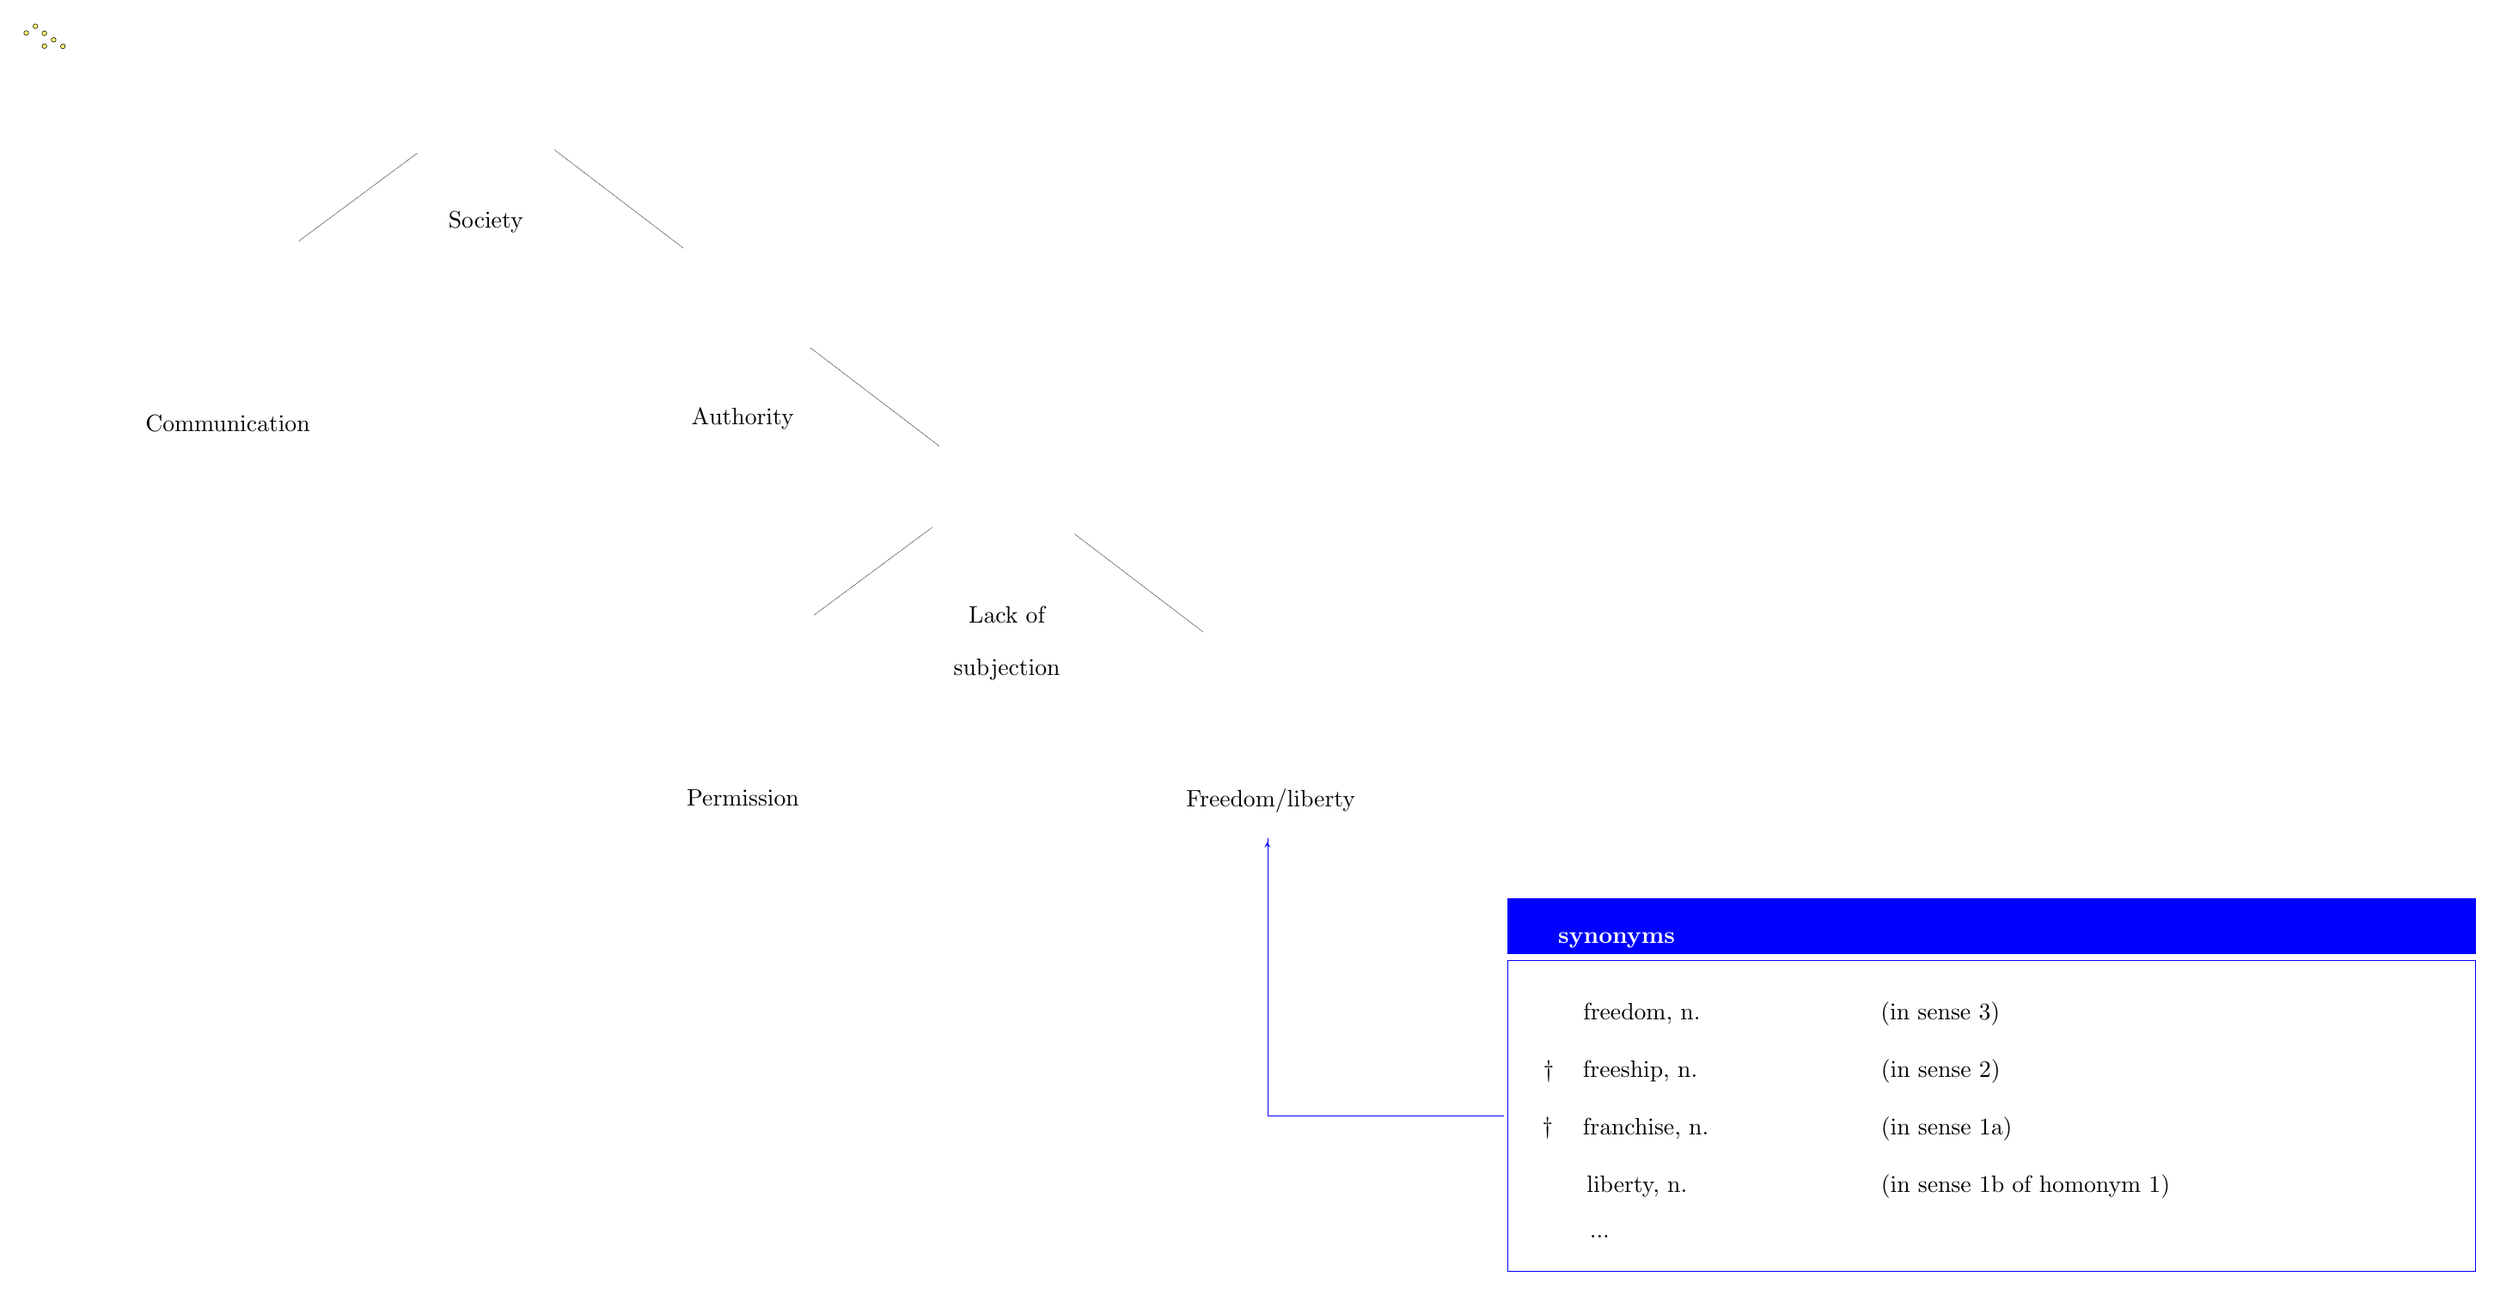
\begin{tikzpicture}
\pgftransformxscale{1.000000}
\pgftransformyscale{-1.000000}
\definecolor{dialinecolor}{rgb}{0.000000, 0.000000, 0.000000}
\pgfsetstrokecolor{dialinecolor}
\definecolor{dialinecolor}{rgb}{1.000000, 1.000000, 1.000000}
\pgfsetfillcolor{dialinecolor}
\pgfsetlinewidth{0.100000\du}
\pgfsetdash{}{0pt}
\pgfsetdash{}{0pt}
\pgfsetbuttcap
\pgfsetmiterjoin
\pgfsetlinewidth{0.100000\du}
\pgfsetbuttcap
\pgfsetmiterjoin
\pgfsetdash{}{0pt}
\definecolor{dialinecolor}{rgb}{1.000000, 0.984314, 0.435294}
\pgfsetfillcolor{dialinecolor}
\pgfpathellipse{\pgfpoint{14.600000\du}{6.900000\du}}{\pgfpoint{1.000000\du}{0\du}}{\pgfpoint{0\du}{1.000000\du}}
\pgfusepath{fill}
\definecolor{dialinecolor}{rgb}{0.000000, 0.000000, 0.000000}
\pgfsetstrokecolor{dialinecolor}
\pgfpathellipse{\pgfpoint{14.600000\du}{6.900000\du}}{\pgfpoint{1.000000\du}{0\du}}{\pgfpoint{0\du}{1.000000\du}}
\pgfusepath{stroke}
\pgfsetbuttcap
\pgfsetmiterjoin
\pgfsetdash{}{0pt}
\definecolor{dialinecolor}{rgb}{0.000000, 0.000000, 0.000000}
\pgfsetstrokecolor{dialinecolor}
\pgfpathellipse{\pgfpoint{14.600000\du}{6.900000\du}}{\pgfpoint{1.000000\du}{0\du}}{\pgfpoint{0\du}{1.000000\du}}
\pgfusepath{stroke}
\pgfsetlinewidth{0.100000\du}
\pgfsetdash{}{0pt}
\pgfsetdash{}{0pt}
\pgfsetmiterjoin
\definecolor{dialinecolor}{rgb}{1.000000, 1.000000, 1.000000}
\pgfsetfillcolor{dialinecolor}
\fill (22.000000\du,13.850000\du)--(22.000000\du,18.450000\du)--(36.300000\du,18.450000\du)--(36.300000\du,13.850000\du)--cycle;
\definecolor{dialinecolor}{rgb}{0.000000, 0.000000, 1.000000}
\pgfsetstrokecolor{dialinecolor}
\draw (22.000000\du,13.850000\du)--(22.000000\du,18.450000\du)--(36.300000\du,18.450000\du)--(36.300000\du,13.850000\du)--cycle;
% setfont left to latex
\definecolor{dialinecolor}{rgb}{0.000000, 0.000000, 0.000000}
\pgfsetstrokecolor{dialinecolor}
\node[anchor=west] at (23.050000\du,17.200000\du){liberty, n.};
% setfont left to latex
\definecolor{dialinecolor}{rgb}{0.000000, 0.000000, 0.000000}
\pgfsetstrokecolor{dialinecolor}
\node[anchor=west] at (23.000000\du,14.650000\du){freedom, n.};
\pgfsetlinewidth{0.100000\du}
\pgfsetdash{}{0pt}
\pgfsetdash{}{0pt}
\pgfsetmiterjoin
\pgfsetbuttcap
{
\definecolor{dialinecolor}{rgb}{0.000000, 0.000000, 1.000000}
\pgfsetfillcolor{dialinecolor}
% was here!!!
\pgfsetarrowsend{stealth}
{\pgfsetcornersarced{\pgfpoint{0.000000\du}{0.000000\du}}\definecolor{dialinecolor}{rgb}{0.000000, 0.000000, 1.000000}
\pgfsetstrokecolor{dialinecolor}
\draw (21.949713\du,16.150000\du)--(18.450000\du,16.150000\du)--(18.450000\du,12.100000\du)--(18.450000\du,12.100000\du);
}}
\definecolor{dialinecolor}{rgb}{1.000000, 1.000000, 1.000000}
\pgfsetfillcolor{dialinecolor}
\fill (16.050000\du,13.805000\du)--(16.050000\du,14.550000\du)--(16.050000\du,14.550000\du)--(16.050000\du,13.805000\du)--cycle;
% setfont left to latex
\definecolor{dialinecolor}{rgb}{0.000000, 0.000000, 0.000000}
\pgfsetstrokecolor{dialinecolor}
\node at (16.050000\du,14.400000\du){};
\definecolor{dialinecolor}{rgb}{1.000000, 1.000000, 1.000000}
\pgfsetfillcolor{dialinecolor}
\fill (12.726250\du,8.155000\du)--(12.726250\du,9.700000\du)--(16.473750\du,9.700000\du)--(16.473750\du,8.155000\du)--cycle;
% setfont left to latex
\definecolor{dialinecolor}{rgb}{0.000000, 0.000000, 0.000000}
\pgfsetstrokecolor{dialinecolor}
\node at (14.600000\du,8.750000\du){Lack of };
% setfont left to latex
\definecolor{dialinecolor}{rgb}{0.000000, 0.000000, 0.000000}
\pgfsetstrokecolor{dialinecolor}
\node at (14.600000\du,9.550000\du){subjection};
\pgfsetlinewidth{0.100000\du}
\pgfsetdash{}{0pt}
\pgfsetdash{}{0pt}
\pgfsetbuttcap
\pgfsetmiterjoin
\pgfsetlinewidth{0.100000\du}
\pgfsetbuttcap
\pgfsetmiterjoin
\pgfsetdash{}{0pt}
\definecolor{dialinecolor}{rgb}{1.000000, 0.984314, 0.435294}
\pgfsetfillcolor{dialinecolor}
\pgfpathellipse{\pgfpoint{10.695000\du}{4.150000\du}}{\pgfpoint{1.000000\du}{0\du}}{\pgfpoint{0\du}{1.000000\du}}
\pgfusepath{fill}
\definecolor{dialinecolor}{rgb}{0.000000, 0.000000, 0.000000}
\pgfsetstrokecolor{dialinecolor}
\pgfpathellipse{\pgfpoint{10.695000\du}{4.150000\du}}{\pgfpoint{1.000000\du}{0\du}}{\pgfpoint{0\du}{1.000000\du}}
\pgfusepath{stroke}
\pgfsetbuttcap
\pgfsetmiterjoin
\pgfsetdash{}{0pt}
\definecolor{dialinecolor}{rgb}{0.000000, 0.000000, 0.000000}
\pgfsetstrokecolor{dialinecolor}
\pgfpathellipse{\pgfpoint{10.695000\du}{4.150000\du}}{\pgfpoint{1.000000\du}{0\du}}{\pgfpoint{0\du}{1.000000\du}}
\pgfusepath{stroke}
\pgfsetlinewidth{0.100000\du}
\pgfsetdash{}{0pt}
\pgfsetdash{}{0pt}
\pgfsetbuttcap
\pgfsetmiterjoin
\pgfsetlinewidth{0.100000\du}
\pgfsetbuttcap
\pgfsetmiterjoin
\pgfsetdash{}{0pt}
\definecolor{dialinecolor}{rgb}{1.000000, 0.984314, 0.435294}
\pgfsetfillcolor{dialinecolor}
\pgfpathellipse{\pgfpoint{6.940000\du}{1.200000\du}}{\pgfpoint{1.000000\du}{0\du}}{\pgfpoint{0\du}{1.000000\du}}
\pgfusepath{fill}
\definecolor{dialinecolor}{rgb}{0.000000, 0.000000, 0.000000}
\pgfsetstrokecolor{dialinecolor}
\pgfpathellipse{\pgfpoint{6.940000\du}{1.200000\du}}{\pgfpoint{1.000000\du}{0\du}}{\pgfpoint{0\du}{1.000000\du}}
\pgfusepath{stroke}
\pgfsetbuttcap
\pgfsetmiterjoin
\pgfsetdash{}{0pt}
\definecolor{dialinecolor}{rgb}{0.000000, 0.000000, 0.000000}
\pgfsetstrokecolor{dialinecolor}
\pgfpathellipse{\pgfpoint{6.940000\du}{1.200000\du}}{\pgfpoint{1.000000\du}{0\du}}{\pgfpoint{0\du}{1.000000\du}}
\pgfusepath{stroke}
\definecolor{dialinecolor}{rgb}{1.000000, 1.000000, 1.000000}
\pgfsetfillcolor{dialinecolor}
\fill (8.991250\du,5.250000\du)--(8.991250\du,5.995000\du)--(12.398750\du,5.995000\du)--(12.398750\du,5.250000\du)--cycle;
% setfont left to latex
\definecolor{dialinecolor}{rgb}{0.000000, 0.000000, 0.000000}
\pgfsetstrokecolor{dialinecolor}
\node at (10.695000\du,5.845000\du){Authority};
\definecolor{dialinecolor}{rgb}{1.000000, 1.000000, 1.000000}
\pgfsetfillcolor{dialinecolor}
\fill (5.570000\du,2.350000\du)--(5.570000\du,3.095000\du)--(8.227500\du,3.095000\du)--(8.227500\du,2.350000\du)--cycle;
% setfont left to latex
\definecolor{dialinecolor}{rgb}{0.000000, 0.000000, 0.000000}
\pgfsetstrokecolor{dialinecolor}
\node at (6.898750\du,2.945000\du){Society};
\pgfsetlinewidth{0.100000\du}
\pgfsetdash{}{0pt}
\pgfsetdash{}{0pt}
\pgfsetbuttcap
{
\definecolor{dialinecolor}{rgb}{0.000000, 0.000000, 0.000000}
\pgfsetfillcolor{dialinecolor}
% was here!!!
\definecolor{dialinecolor}{rgb}{0.000000, 0.000000, 0.000000}
\pgfsetstrokecolor{dialinecolor}
\draw (13.600000\du,6.250000\du)--(11.700000\du,4.800000\du);
}
\pgfsetlinewidth{0.100000\du}
\pgfsetdash{}{0pt}
\pgfsetdash{}{0pt}
\pgfsetbuttcap
{
\definecolor{dialinecolor}{rgb}{0.000000, 0.000000, 0.000000}
\pgfsetfillcolor{dialinecolor}
% was here!!!
\definecolor{dialinecolor}{rgb}{0.000000, 0.000000, 0.000000}
\pgfsetstrokecolor{dialinecolor}
\draw (9.815080\du,3.320080\du)--(7.915080\du,1.870080\du);
}
\pgfsetlinewidth{0.100000\du}
\pgfsetdash{}{0pt}
\pgfsetdash{}{0pt}
\pgfsetmiterjoin
\definecolor{dialinecolor}{rgb}{0.000000, 0.000000, 1.000000}
\pgfsetfillcolor{dialinecolor}
\fill (21.997400\du,12.943200\du)--(21.997400\du,13.755370\du)--(36.300100\du,13.755370\du)--(36.300100\du,12.943200\du)--cycle;
\definecolor{dialinecolor}{rgb}{0.000000, 0.000000, 1.000000}
\pgfsetstrokecolor{dialinecolor}
\draw (21.997400\du,12.943200\du)--(21.997400\du,13.755370\du)--(36.300100\du,13.755370\du)--(36.300100\du,12.943200\du)--cycle;
% setfont left to latex
\definecolor{dialinecolor}{rgb}{1.000000, 1.000000, 1.000000}
\pgfsetstrokecolor{dialinecolor}
\node[anchor=west,white] at (22.629800\du,13.562800\du){\textbf{\textcolor{white}{synonyms}}};
\pgfsetlinewidth{0.100000\du}
\pgfsetdash{}{0pt}
\pgfsetdash{}{0pt}
\pgfsetbuttcap
\pgfsetmiterjoin
\pgfsetlinewidth{0.100000\du}
\pgfsetbuttcap
\pgfsetmiterjoin
\pgfsetdash{}{0pt}
\definecolor{dialinecolor}{rgb}{1.000000, 0.984314, 0.435294}
\pgfsetfillcolor{dialinecolor}
\pgfpathellipse{\pgfpoint{18.500000\du}{9.650000\du}}{\pgfpoint{1.000000\du}{0\du}}{\pgfpoint{0\du}{1.000000\du}}
\pgfusepath{fill}
\definecolor{dialinecolor}{rgb}{0.000000, 0.000000, 0.000000}
\pgfsetstrokecolor{dialinecolor}
\pgfpathellipse{\pgfpoint{18.500000\du}{9.650000\du}}{\pgfpoint{1.000000\du}{0\du}}{\pgfpoint{0\du}{1.000000\du}}
\pgfusepath{stroke}
\pgfsetbuttcap
\pgfsetmiterjoin
\pgfsetdash{}{0pt}
\definecolor{dialinecolor}{rgb}{0.000000, 0.000000, 0.000000}
\pgfsetstrokecolor{dialinecolor}
\pgfpathellipse{\pgfpoint{18.500000\du}{9.650000\du}}{\pgfpoint{1.000000\du}{0\du}}{\pgfpoint{0\du}{1.000000\du}}
\pgfusepath{stroke}
\definecolor{dialinecolor}{rgb}{1.000000, 1.000000, 1.000000}
\pgfsetfillcolor{dialinecolor}
\fill (15.603750\du,10.905000\du)--(15.603750\du,11.650000\du)--(21.396250\du,11.650000\du)--(21.396250\du,10.905000\du)--cycle;
% setfont left to latex
\definecolor{dialinecolor}{rgb}{0.000000, 0.000000, 0.000000}
\pgfsetstrokecolor{dialinecolor}
\node at (18.500000\du,11.500000\du){Freedom/liberty};
\pgfsetlinewidth{0.100000\du}
\pgfsetdash{}{0pt}
\pgfsetdash{}{0pt}
\pgfsetbuttcap
{
\definecolor{dialinecolor}{rgb}{0.000000, 0.000000, 0.000000}
\pgfsetfillcolor{dialinecolor}
% was here!!!
\definecolor{dialinecolor}{rgb}{0.000000, 0.000000, 0.000000}
\pgfsetstrokecolor{dialinecolor}
\draw (17.500000\du,9.000000\du)--(15.600000\du,7.550000\du);
}
% setfont left to latex
\definecolor{dialinecolor}{rgb}{0.000000, 0.000000, 0.000000}
\pgfsetstrokecolor{dialinecolor}
\node[anchor=west] at (22.995000\du,15.495000\du){freeship, n.};
% setfont left to latex
\definecolor{dialinecolor}{rgb}{0.000000, 0.000000, 0.000000}
\pgfsetstrokecolor{dialinecolor}
\node[anchor=west] at (22.995000\du,16.345000\du){franchise, n.};
% setfont left to latex
\definecolor{dialinecolor}{rgb}{0.000000, 0.000000, 0.000000}
\pgfsetstrokecolor{dialinecolor}
\node[anchor=west] at (23.095000\du,17.945000\du){...};
% setfont left to latex
\definecolor{dialinecolor}{rgb}{0.000000, 0.000000, 0.000000}
\pgfsetstrokecolor{dialinecolor}
\node[anchor=west] at (27.395000\du,14.645000\du){(in sense 3)};
\pgfsetlinewidth{0.100000\du}
\pgfsetdash{}{0pt}
\pgfsetdash{}{0pt}
\pgfsetbuttcap
{
\definecolor{dialinecolor}{rgb}{0.000000, 0.000000, 0.000000}
\pgfsetfillcolor{dialinecolor}
% was here!!!
\definecolor{dialinecolor}{rgb}{0.000000, 0.000000, 0.000000}
\pgfsetstrokecolor{dialinecolor}
\draw (13.500000\du,7.450000\du)--(11.750000\du,8.750000\du);
}
\pgfsetlinewidth{0.100000\du}
\pgfsetdash{}{0pt}
\pgfsetdash{}{0pt}
\pgfsetbuttcap
\pgfsetmiterjoin
\pgfsetlinewidth{0.100000\du}
\pgfsetbuttcap
\pgfsetmiterjoin
\pgfsetdash{}{0pt}
\definecolor{dialinecolor}{rgb}{1.000000, 0.984314, 0.435294}
\pgfsetfillcolor{dialinecolor}
\pgfpathellipse{\pgfpoint{10.715080\du}{9.570080\du}}{\pgfpoint{1.000000\du}{0\du}}{\pgfpoint{0\du}{1.000000\du}}
\pgfusepath{fill}
\definecolor{dialinecolor}{rgb}{0.000000, 0.000000, 0.000000}
\pgfsetstrokecolor{dialinecolor}
\pgfpathellipse{\pgfpoint{10.715080\du}{9.570080\du}}{\pgfpoint{1.000000\du}{0\du}}{\pgfpoint{0\du}{1.000000\du}}
\pgfusepath{stroke}
\pgfsetbuttcap
\pgfsetmiterjoin
\pgfsetdash{}{0pt}
\definecolor{dialinecolor}{rgb}{0.000000, 0.000000, 0.000000}
\pgfsetstrokecolor{dialinecolor}
\pgfpathellipse{\pgfpoint{10.715080\du}{9.570080\du}}{\pgfpoint{1.000000\du}{0\du}}{\pgfpoint{0\du}{1.000000\du}}
\pgfusepath{stroke}
\definecolor{dialinecolor}{rgb}{1.000000, 1.000000, 1.000000}
\pgfsetfillcolor{dialinecolor}
\fill (8.708750\du,10.855000\du)--(8.708750\du,11.600000\du)--(12.691250\du,11.600000\du)--(12.691250\du,10.855000\du)--cycle;
% setfont left to latex
\definecolor{dialinecolor}{rgb}{0.000000, 0.000000, 0.000000}
\pgfsetstrokecolor{dialinecolor}
\node at (10.700000\du,11.450000\du){Permission};
\pgfsetlinewidth{0.100000\du}
\pgfsetdash{}{0pt}
\pgfsetdash{}{0pt}
\pgfsetbuttcap
{
\definecolor{dialinecolor}{rgb}{0.000000, 0.000000, 0.000000}
\pgfsetfillcolor{dialinecolor}
% was here!!!
\definecolor{dialinecolor}{rgb}{0.000000, 0.000000, 0.000000}
\pgfsetstrokecolor{dialinecolor}
\draw (5.886250\du,1.919950\du)--(4.136250\du,3.219950\du);
}
\pgfsetlinewidth{0.100000\du}
\pgfsetdash{}{0pt}
\pgfsetdash{}{0pt}
\pgfsetbuttcap
\pgfsetmiterjoin
\pgfsetlinewidth{0.100000\du}
\pgfsetbuttcap
\pgfsetmiterjoin
\pgfsetdash{}{0pt}
\definecolor{dialinecolor}{rgb}{1.000000, 0.984314, 0.435294}
\pgfsetfillcolor{dialinecolor}
\pgfpathellipse{\pgfpoint{3.101330\du}{4.040030\du}}{\pgfpoint{1.000000\du}{0\du}}{\pgfpoint{0\du}{1.000000\du}}
\pgfusepath{fill}
\definecolor{dialinecolor}{rgb}{0.000000, 0.000000, 0.000000}
\pgfsetstrokecolor{dialinecolor}
\pgfpathellipse{\pgfpoint{3.101330\du}{4.040030\du}}{\pgfpoint{1.000000\du}{0\du}}{\pgfpoint{0\du}{1.000000\du}}
\pgfusepath{stroke}
\pgfsetbuttcap
\pgfsetmiterjoin
\pgfsetdash{}{0pt}
\definecolor{dialinecolor}{rgb}{0.000000, 0.000000, 0.000000}
\pgfsetstrokecolor{dialinecolor}
\pgfpathellipse{\pgfpoint{3.101330\du}{4.040030\du}}{\pgfpoint{1.000000\du}{0\du}}{\pgfpoint{0\du}{1.000000\du}}
\pgfusepath{stroke}
\definecolor{dialinecolor}{rgb}{1.000000, 1.000000, 1.000000}
\pgfsetfillcolor{dialinecolor}
\fill (0.282500\du,5.324950\du)--(0.282500\du,6.069950\du)--(5.890000\du,6.069950\du)--(5.890000\du,5.324950\du)--cycle;
% setfont left to latex
\definecolor{dialinecolor}{rgb}{0.000000, 0.000000, 0.000000}
\pgfsetstrokecolor{dialinecolor}
\node at (3.086250\du,5.919950\du){Communication};
% setfont left to latex
\definecolor{dialinecolor}{rgb}{0.000000, 0.000000, 0.000000}
\pgfsetstrokecolor{dialinecolor}
\node[anchor=west] at (27.400000\du,15.500000\du){(in sense 2)};
% setfont left to latex
\definecolor{dialinecolor}{rgb}{0.000000, 0.000000, 0.000000}
\pgfsetstrokecolor{dialinecolor}
\node[anchor=west] at (27.400000\du,16.350000\du){(in sense 1a)};
% setfont left to latex
\definecolor{dialinecolor}{rgb}{0.000000, 0.000000, 0.000000}
\pgfsetstrokecolor{dialinecolor}
\node[anchor=west] at (27.400000\du,17.200000\du){(in sense 1b of homonym 1)};
% setfont left to latex
\definecolor{dialinecolor}{rgb}{0.000000, 0.000000, 0.000000}
\pgfsetstrokecolor{dialinecolor}
\node[anchor=west] at (22.410000\du,15.495000\du){$\dagger$};
% setfont left to latex
\definecolor{dialinecolor}{rgb}{0.000000, 0.000000, 0.000000}
\pgfsetstrokecolor{dialinecolor}
\node[anchor=west] at (22.395000\du,16.340000\du){$\dagger$};
\end{tikzpicture}

		}
	}
	\caption[]{\label{fig:Stolk2017:HTE} Example HTOED content based on  \cite{kay_historical_2010}}
\end{figure} 

Expressing categories of the topical system of HTOED in OntoLex is relatively straightforward. Each HTOED category corresponds with a lexical concept in OntoLex. The latter is defined as a ``mental abstraction, concept or unit of thought that can be lexicalized by a given collection of senses'' \cite{cimiano_lexicon_2016}. This definition appears highly applicable to categories from topical thesauri. As lexical concepts are asserted to be specializations of SKOS concepts, it is possible to capture the hierarchy between categories using the \texttt{broader}/\texttt{narrower} relations from SKOS \cite{miles_skos_2009}. Listing \ref{lst:Stolk2017:HTE-cat} contains the RDF for expressing one of the HTOED categories in OntoLex, ``Freedom/Liberty'', and the relation to its superordinate category ``Lack of subjection''.

\noindent
\begin{minipage}[c]{\textwidth}
	\begin{lstlisting}[
		caption={HTOED category ``Freedom/liberty'' expressed in OntoLex},
		label={lst:Stolk2017:HTE-cat}
	]
<category-FreedomLiberty> a ontolex:LexicalConcept ;
	skos:prefLabel "Freedom/liberty"@en ;
	skos:broader <category-LackOfSubjection> .
	\end{lstlisting}
\end{minipage}

The OntoLex vocabulary also contains terminology to express lexical senses and the lexical entries to which they belong. In order to state that a given lexical sense from HTOED belongs to one of its categories, the property \texttt{ontolex:isLexicalizedSenseOf} can be used. This property relates a lexical sense to a lexical concept, stating that it ``lexicalizes'' that concept. According to the section on Lexical Nets in the OntoLex specification, lexical senses that lexicalize the same concept are considered synonymous \cite{cimiano_lexicon_2016}. In other words, the relation of synonymy is not explicitly asserted in OntoLex, but can be inferred from the use of the \texttt{ontolex:isLexicalizedSenseOf} property. The resulting RDF for the sense of \textit{freedom} from the HTOED sample and its relation to the ``Freedom/liberty'' category is provided in Listing \ref{lst:Stolk2017:HTE-sense}.

\noindent
\begin{minipage}[c]{\textwidth}
	\begin{lstlisting}[
		caption={HTOED sense of \textit{freedom} expressed in OntoLex},
		label={lst:Stolk2017:HTE-sense}
	]
<sense-freedom-n-3> a ontolex:LexicalSense ;
	skos:prefLabel "freedom n. (sense 3)"@en ;
	ontolex:isSenseOf <entry-freedom-n> ;
	ontolex:isLexicalizedSenseOf <category-FreedomLiberty> .

<entry-freedom-n> a ontolex:LexicalEntry ;
	skos:prefLabel "freedom, n."@en ;
	wn:partOfSpeech wn:noun .
	\end{lstlisting}
\end{minipage}
 
As shown, capturing the onomasiological ordering of the HTOED lexicon presents no issues with the OntoLex vocabulary. The vocabulary enables one to express categories and their hierarchy, lexical senses and their relation to a lexical entry, and the relation between the senses from HTOED and the categories to which they belong.


\section{Case study \textit{The Scots Thesaurus}}

The second case study in this paper concerns \textit{The Scots Thesaurus} (ScT) \cite{macleod_scots_1990}. ScT captures the Lowland Scots lexis available throughout history, from its twelfth-century beginnings to the present. This thesaurus, published in 1990, categorizes its lexical items but does not indicate synonymy. Figure \ref{fig:Stolk2017:ScT} depicts the sample taken from ScT, encompassing five categories and four lexical senses.

% Dia export had to be mended slightly:
% - dagger symbol did not appear (replaced † with $\dagger$)
\begin{figure}[htbp]
	\framebox[\textwidth]{
		\scalebox{0.65}[0.65]{
			% Graphic for TeX using PGF
% Title: C:\Users\Sander\Documents\Dropbox\PhD\images\Content-parts (ScT-2).dia
% Creator: Dia v0.97.2
% CreationDate: Sun Apr 02 17:48:04 2017
% For: Sander
% \usepackage{tikz}
% The following commands are not supported in PSTricks at present
% We define them conditionally, so when they are implemented,
% this pgf file will use them.
\ifx\du\undefined
  \newlength{\du}
\fi
\setlength{\du}{15\unitlength}
\begin{tikzpicture}
\pgftransformxscale{1.000000}
\pgftransformyscale{-1.000000}
\definecolor{dialinecolor}{rgb}{0.000000, 0.000000, 0.000000}
\pgfsetstrokecolor{dialinecolor}
\definecolor{dialinecolor}{rgb}{1.000000, 1.000000, 1.000000}
\pgfsetfillcolor{dialinecolor}
\pgfsetlinewidth{0.100000\du}
\pgfsetdash{}{0pt}
\pgfsetdash{}{0pt}
\pgfsetmiterjoin
\definecolor{dialinecolor}{rgb}{1.000000, 1.000000, 1.000000}
\pgfsetfillcolor{dialinecolor}
\fill (18.100000\du,11.000000\du)--(18.100000\du,15.600000\du)--(32.871967\du,15.600000\du)--(32.871967\du,11.000000\du)--cycle;
\definecolor{dialinecolor}{rgb}{0.000000, 0.000000, 1.000000}
\pgfsetstrokecolor{dialinecolor}
\draw (18.100000\du,11.000000\du)--(18.100000\du,15.600000\du)--(32.871967\du,15.600000\du)--(32.871967\du,11.000000\du)--cycle;
% setfont left to latex
\definecolor{dialinecolor}{rgb}{0.000000, 0.000000, 0.000000}
\pgfsetstrokecolor{dialinecolor}
\node[anchor=west] at (19.150000\du,14.350000\du){miss};
% setfont left to latex
\definecolor{dialinecolor}{rgb}{0.000000, 0.000000, 0.000000}
\pgfsetstrokecolor{dialinecolor}
\node[anchor=west] at (19.100000\du,11.800000\du){blander};
\pgfsetlinewidth{0.100000\du}
\pgfsetdash{}{0pt}
\pgfsetdash{}{0pt}
\pgfsetmiterjoin
\pgfsetbuttcap
{
\definecolor{dialinecolor}{rgb}{0.000000, 0.000000, 1.000000}
\pgfsetfillcolor{dialinecolor}
% was here!!!
\pgfsetarrowsend{stealth}
{\pgfsetcornersarced{\pgfpoint{0.000000\du}{0.000000\du}}\definecolor{dialinecolor}{rgb}{0.000000, 0.000000, 1.000000}
\pgfsetstrokecolor{dialinecolor}
\draw (18.049928\du,13.300000\du)--(14.550000\du,13.300000\du)--(14.550000\du,9.250000\du)--(14.550000\du,9.250000\du);
}}
\definecolor{dialinecolor}{rgb}{1.000000, 1.000000, 1.000000}
\pgfsetfillcolor{dialinecolor}
\fill (12.150000\du,10.955000\du)--(12.150000\du,11.700000\du)--(12.150000\du,11.700000\du)--(12.150000\du,10.955000\du)--cycle;
% setfont left to latex
\definecolor{dialinecolor}{rgb}{0.000000, 0.000000, 0.000000}
\pgfsetstrokecolor{dialinecolor}
\node at (12.150000\du,11.550000\du){};
\pgfsetlinewidth{0.100000\du}
\pgfsetdash{}{0pt}
\pgfsetdash{}{0pt}
\pgfsetbuttcap
\pgfsetmiterjoin
\pgfsetlinewidth{0.100000\du}
\pgfsetbuttcap
\pgfsetmiterjoin
\pgfsetdash{}{0pt}
\definecolor{dialinecolor}{rgb}{1.000000, 0.984314, 0.435294}
\pgfsetfillcolor{dialinecolor}
\pgfpathellipse{\pgfpoint{10.695000\du}{4.150000\du}}{\pgfpoint{1.000000\du}{0\du}}{\pgfpoint{0\du}{1.000000\du}}
\pgfusepath{fill}
\definecolor{dialinecolor}{rgb}{0.000000, 0.000000, 0.000000}
\pgfsetstrokecolor{dialinecolor}
\pgfpathellipse{\pgfpoint{10.695000\du}{4.150000\du}}{\pgfpoint{1.000000\du}{0\du}}{\pgfpoint{0\du}{1.000000\du}}
\pgfusepath{stroke}
\pgfsetbuttcap
\pgfsetmiterjoin
\pgfsetdash{}{0pt}
\definecolor{dialinecolor}{rgb}{0.000000, 0.000000, 0.000000}
\pgfsetstrokecolor{dialinecolor}
\pgfpathellipse{\pgfpoint{10.695000\du}{4.150000\du}}{\pgfpoint{1.000000\du}{0\du}}{\pgfpoint{0\du}{1.000000\du}}
\pgfusepath{stroke}
\pgfsetlinewidth{0.100000\du}
\pgfsetdash{}{0pt}
\pgfsetdash{}{0pt}
\pgfsetbuttcap
\pgfsetmiterjoin
\pgfsetlinewidth{0.100000\du}
\pgfsetbuttcap
\pgfsetmiterjoin
\pgfsetdash{}{0pt}
\definecolor{dialinecolor}{rgb}{1.000000, 0.984314, 0.435294}
\pgfsetfillcolor{dialinecolor}
\pgfpathellipse{\pgfpoint{6.940000\du}{1.200000\du}}{\pgfpoint{1.000000\du}{0\du}}{\pgfpoint{0\du}{1.000000\du}}
\pgfusepath{fill}
\definecolor{dialinecolor}{rgb}{0.000000, 0.000000, 0.000000}
\pgfsetstrokecolor{dialinecolor}
\pgfpathellipse{\pgfpoint{6.940000\du}{1.200000\du}}{\pgfpoint{1.000000\du}{0\du}}{\pgfpoint{0\du}{1.000000\du}}
\pgfusepath{stroke}
\pgfsetbuttcap
\pgfsetmiterjoin
\pgfsetdash{}{0pt}
\definecolor{dialinecolor}{rgb}{0.000000, 0.000000, 0.000000}
\pgfsetstrokecolor{dialinecolor}
\pgfpathellipse{\pgfpoint{6.940000\du}{1.200000\du}}{\pgfpoint{1.000000\du}{0\du}}{\pgfpoint{0\du}{1.000000\du}}
\pgfusepath{stroke}
\definecolor{dialinecolor}{rgb}{1.000000, 1.000000, 1.000000}
\pgfsetfillcolor{dialinecolor}
\fill (9.663750\du,5.250000\du)--(9.663750\du,5.995000\du)--(11.726250\du,5.995000\du)--(11.726250\du,5.250000\du)--cycle;
% setfont left to latex
\definecolor{dialinecolor}{rgb}{0.000000, 0.000000, 0.000000}
\pgfsetstrokecolor{dialinecolor}
\node at (10.695000\du,5.845000\du){Crops};
\definecolor{dialinecolor}{rgb}{1.000000, 1.000000, 1.000000}
\pgfsetfillcolor{dialinecolor}
\fill (5.406250\du,2.350000\du)--(5.406250\du,3.095000\du)--(8.391250\du,3.095000\du)--(8.391250\du,2.350000\du)--cycle;
% setfont left to latex
\definecolor{dialinecolor}{rgb}{0.000000, 0.000000, 0.000000}
\pgfsetstrokecolor{dialinecolor}
\node at (6.898750\du,2.945000\du){Farming};
\pgfsetlinewidth{0.100000\du}
\pgfsetdash{}{0pt}
\pgfsetdash{}{0pt}
\pgfsetbuttcap
{
\definecolor{dialinecolor}{rgb}{0.000000, 0.000000, 0.000000}
\pgfsetfillcolor{dialinecolor}
% was here!!!
\definecolor{dialinecolor}{rgb}{0.000000, 0.000000, 0.000000}
\pgfsetstrokecolor{dialinecolor}
\draw (9.815080\du,3.320080\du)--(7.915080\du,1.870080\du);
}
\pgfsetlinewidth{0.100000\du}
\pgfsetdash{}{0pt}
\pgfsetdash{}{0pt}
\pgfsetbuttcap
\pgfsetmiterjoin
\pgfsetlinewidth{0.100000\du}
\pgfsetbuttcap
\pgfsetmiterjoin
\pgfsetdash{}{0pt}
\definecolor{dialinecolor}{rgb}{1.000000, 0.984314, 0.435294}
\pgfsetfillcolor{dialinecolor}
\pgfpathellipse{\pgfpoint{14.600000\du}{7.050000\du}}{\pgfpoint{1.000000\du}{0\du}}{\pgfpoint{0\du}{1.000000\du}}
\pgfusepath{fill}
\definecolor{dialinecolor}{rgb}{0.000000, 0.000000, 0.000000}
\pgfsetstrokecolor{dialinecolor}
\pgfpathellipse{\pgfpoint{14.600000\du}{7.050000\du}}{\pgfpoint{1.000000\du}{0\du}}{\pgfpoint{0\du}{1.000000\du}}
\pgfusepath{stroke}
\pgfsetbuttcap
\pgfsetmiterjoin
\pgfsetdash{}{0pt}
\definecolor{dialinecolor}{rgb}{0.000000, 0.000000, 0.000000}
\pgfsetstrokecolor{dialinecolor}
\pgfpathellipse{\pgfpoint{14.600000\du}{7.050000\du}}{\pgfpoint{1.000000\du}{0\du}}{\pgfpoint{0\du}{1.000000\du}}
\pgfusepath{stroke}
\definecolor{dialinecolor}{rgb}{1.000000, 1.000000, 1.000000}
\pgfsetfillcolor{dialinecolor}
\fill (13.237500\du,8.305000\du)--(13.237500\du,9.050000\du)--(15.862500\du,9.050000\du)--(15.862500\du,8.305000\du)--cycle;
% setfont left to latex
\definecolor{dialinecolor}{rgb}{0.000000, 0.000000, 0.000000}
\pgfsetstrokecolor{dialinecolor}
\node at (14.550000\du,8.900000\du){Sowing};
\pgfsetlinewidth{0.100000\du}
\pgfsetdash{}{0pt}
\pgfsetdash{}{0pt}
\pgfsetbuttcap
{
\definecolor{dialinecolor}{rgb}{0.000000, 0.000000, 0.000000}
\pgfsetfillcolor{dialinecolor}
% was here!!!
\definecolor{dialinecolor}{rgb}{0.000000, 0.000000, 0.000000}
\pgfsetstrokecolor{dialinecolor}
\draw (13.600000\du,6.400000\du)--(11.700000\du,4.950000\du);
}
% setfont left to latex
\definecolor{dialinecolor}{rgb}{0.000000, 0.000000, 0.000000}
\pgfsetstrokecolor{dialinecolor}
\node[anchor=west] at (19.095000\du,12.645000\du){happer};
% setfont left to latex
\definecolor{dialinecolor}{rgb}{0.000000, 0.000000, 0.000000}
\pgfsetstrokecolor{dialinecolor}
\node[anchor=west] at (19.095000\du,13.495000\du){heuch};
% setfont left to latex
\definecolor{dialinecolor}{rgb}{0.000000, 0.000000, 0.000000}
\pgfsetstrokecolor{dialinecolor}
\node[anchor=west] at (19.195000\du,15.095000\du){...};
% setfont left to latex
\definecolor{dialinecolor}{rgb}{0.000000, 0.000000, 0.000000}
\pgfsetstrokecolor{dialinecolor}
\node[anchor=west] at (22.036057\du,11.795000\du){(in sense 'disperse scantily')};
\pgfsetlinewidth{0.100000\du}
\pgfsetdash{}{0pt}
\pgfsetdash{}{0pt}
\pgfsetbuttcap
{
\definecolor{dialinecolor}{rgb}{0.000000, 0.000000, 0.000000}
\pgfsetfillcolor{dialinecolor}
% was here!!!
\definecolor{dialinecolor}{rgb}{0.000000, 0.000000, 0.000000}
\pgfsetstrokecolor{dialinecolor}
\draw (9.600000\du,4.850000\du)--(7.850000\du,6.150000\du);
}
\pgfsetlinewidth{0.100000\du}
\pgfsetdash{}{0pt}
\pgfsetdash{}{0pt}
\pgfsetbuttcap
\pgfsetmiterjoin
\pgfsetlinewidth{0.100000\du}
\pgfsetbuttcap
\pgfsetmiterjoin
\pgfsetdash{}{0pt}
\definecolor{dialinecolor}{rgb}{1.000000, 0.984314, 0.435294}
\pgfsetfillcolor{dialinecolor}
\pgfpathellipse{\pgfpoint{6.815080\du}{6.970080\du}}{\pgfpoint{1.000000\du}{0\du}}{\pgfpoint{0\du}{1.000000\du}}
\pgfusepath{fill}
\definecolor{dialinecolor}{rgb}{0.000000, 0.000000, 0.000000}
\pgfsetstrokecolor{dialinecolor}
\pgfpathellipse{\pgfpoint{6.815080\du}{6.970080\du}}{\pgfpoint{1.000000\du}{0\du}}{\pgfpoint{0\du}{1.000000\du}}
\pgfusepath{stroke}
\pgfsetbuttcap
\pgfsetmiterjoin
\pgfsetdash{}{0pt}
\definecolor{dialinecolor}{rgb}{0.000000, 0.000000, 0.000000}
\pgfsetstrokecolor{dialinecolor}
\pgfpathellipse{\pgfpoint{6.815080\du}{6.970080\du}}{\pgfpoint{1.000000\du}{0\du}}{\pgfpoint{0\du}{1.000000\du}}
\pgfusepath{stroke}
\definecolor{dialinecolor}{rgb}{1.000000, 1.000000, 1.000000}
\pgfsetfillcolor{dialinecolor}
\fill (4.985000\du,8.255000\du)--(4.985000\du,9.000000\du)--(8.615000\du,9.000000\du)--(8.615000\du,8.255000\du)--cycle;
% setfont left to latex
\definecolor{dialinecolor}{rgb}{0.000000, 0.000000, 0.000000}
\pgfsetstrokecolor{dialinecolor}
\node at (6.800000\du,8.850000\du){Ploughing};
\pgfsetlinewidth{0.100000\du}
\pgfsetdash{}{0pt}
\pgfsetdash{}{0pt}
\pgfsetbuttcap
{
\definecolor{dialinecolor}{rgb}{0.000000, 0.000000, 0.000000}
\pgfsetfillcolor{dialinecolor}
% was here!!!
\definecolor{dialinecolor}{rgb}{0.000000, 0.000000, 0.000000}
\pgfsetstrokecolor{dialinecolor}
\draw (5.886250\du,1.919950\du)--(4.136250\du,3.219950\du);
}
\pgfsetlinewidth{0.100000\du}
\pgfsetdash{}{0pt}
\pgfsetdash{}{0pt}
\pgfsetbuttcap
\pgfsetmiterjoin
\pgfsetlinewidth{0.100000\du}
\pgfsetbuttcap
\pgfsetmiterjoin
\pgfsetdash{}{0pt}
\definecolor{dialinecolor}{rgb}{1.000000, 0.984314, 0.435294}
\pgfsetfillcolor{dialinecolor}
\pgfpathellipse{\pgfpoint{3.101330\du}{4.040030\du}}{\pgfpoint{1.000000\du}{0\du}}{\pgfpoint{0\du}{1.000000\du}}
\pgfusepath{fill}
\definecolor{dialinecolor}{rgb}{0.000000, 0.000000, 0.000000}
\pgfsetstrokecolor{dialinecolor}
\pgfpathellipse{\pgfpoint{3.101330\du}{4.040030\du}}{\pgfpoint{1.000000\du}{0\du}}{\pgfpoint{0\du}{1.000000\du}}
\pgfusepath{stroke}
\pgfsetbuttcap
\pgfsetmiterjoin
\pgfsetdash{}{0pt}
\definecolor{dialinecolor}{rgb}{0.000000, 0.000000, 0.000000}
\pgfsetstrokecolor{dialinecolor}
\pgfpathellipse{\pgfpoint{3.101330\du}{4.040030\du}}{\pgfpoint{1.000000\du}{0\du}}{\pgfpoint{0\du}{1.000000\du}}
\pgfusepath{stroke}
\definecolor{dialinecolor}{rgb}{1.000000, 1.000000, 1.000000}
\pgfsetfillcolor{dialinecolor}
\fill (1.595000\du,5.324950\du)--(1.595000\du,6.069950\du)--(4.577500\du,6.069950\du)--(4.577500\du,5.324950\du)--cycle;
% setfont left to latex
\definecolor{dialinecolor}{rgb}{0.000000, 0.000000, 0.000000}
\pgfsetstrokecolor{dialinecolor}
\node at (3.086250\du,5.919950\du){Farmers};
% setfont left to latex
\definecolor{dialinecolor}{rgb}{0.000000, 0.000000, 0.000000}
\pgfsetstrokecolor{dialinecolor}
\node[anchor=west] at (22.041057\du,12.650000\du){(in sense 'a basket or container')};
% setfont left to latex
\definecolor{dialinecolor}{rgb}{0.000000, 0.000000, 0.000000}
\pgfsetstrokecolor{dialinecolor}
\node[anchor=west] at (22.041057\du,13.500000\du){(in sense 'earth up plants in drills')};
% setfont left to latex
\definecolor{dialinecolor}{rgb}{0.000000, 0.000000, 0.000000}
\pgfsetstrokecolor{dialinecolor}
\node[anchor=west] at (22.041057\du,14.350000\du){(in sense 'fail to germinate or grow')};
% setfont left to latex
\definecolor{dialinecolor}{rgb}{0.000000, 0.000000, 0.000000}
\pgfsetstrokecolor{dialinecolor}
\node[anchor=west] at (18.510000\du,11.845000\du){$\dagger$};
\end{tikzpicture}

		}
	}
	\caption[]{\label{fig:Stolk2017:ScT} Example ScT content}
\end{figure}

Expressing categories from ScT is possible in a manner identical to that used for HTOED. The result for the ``Sowing'' category from ScT, including its relation to the superordinate category ``Crops'', is provided in Listing \ref{lst:Stolk2017:ScT-cat}.

\noindent
\begin{minipage}[c]{\textwidth}
	\begin{lstlisting}[
		caption={ScT category ``Sowing'' expressed in OntoLex},
		label={lst:Stolk2017:ScT-cat}
	]
<category-Sowing> a ontolex:LexicalConcept ;
	skos:prefLabel "Sowing"@en ;
	skos:broader <category-Crops> .
	\end{lstlisting}
\end{minipage}

As for the lexical senses from ScT, these too can be expressed in OntoLex comparable to how it has been done for HTOED. There is, however, a notable difference. The property \texttt{ontolex:isLexicalizedSenseOf} is unsuitable for relating the senses of ScT to the categories to which they belong. The lexical senses in ScT are not necessarily lexicalizations of the category in question. Moreover, senses that belong to the same category are not necessarily considered synonymous. In fact, they rarely are. A case in point are the senses of \textit{happer} and \textit{miss} from the sample. Both of these senses are members of the category ``Sowing'', and indeed belong to that semantic domain, but can hardly be said to be synonymous or even to lexicalize the category.

What is missing, then, from the OntoLex vocabulary is terminology to express a looser manner of onomasiological ordering with categories than \texttt{ontolex:isLexicalizedSenseOf} does. The RDF snippet in Listing \ref{lst:Stolk2017:ScT-sense} contains the desired situation, where a tentative property \texttt{isSenseIn} is coined (see highlighted line) to express the relation between the sense of \textit{blander} and the category to which it belongs.

\noindent
\begin{minipage}[c]{\textwidth}
	\begin{lstlisting}[
		caption={ScT sense of \textit{blander} expressed in OntoLex},
		label={lst:Stolk2017:ScT-sense}%,
%		linebackgroundcolor={\ifnum\value{lstnumber}=5\color{yellow}\fi} % TODO: fix
	]
<sense-blander-v-disperseScantily> a ontolex:LexicalSense ;
	skos:prefLabel "blander"@sco ;
	skos:definition "disperse scantily"@en ;
	ontolex:isSenseOf <entry-blander-v> ;
	:isSenseIn <category-Sowing> .

<entry-blander-v> a ontolex:LexicalEntry ;
	skos:prefLabel "blander, v."@sco ;
	wn:partOfSpeech wn:noun .
	\end{lstlisting}
\end{minipage}

In short, OntoLex itself does not yet provide terminology to onomasiologically order the lexicographical content of ScT -- and of other thesauri like it.


\section{Discussion}

The two case studies have shown that OntoLex is not yet expressive enough to indicate the relation between senses and categories for all topical thesauri. In fact, the lack of a property like the tentative \texttt{isSenseIn} does not just affect conveying content from ScT and the great many existing cumulative thesauri like it. It also affects expressing these very relations found in thesauri such as HTOED. After all, senses in HTOED are not just lexicalizations of a category, they are also members of a number of categories. To illustrate, the assertion that the HTOED sense of \textit{freedom} is a lexicalization of the category ``Freedom/liberty'' entails that this sense is a member of not just that category but also of its superordinate categories (see Listing \ref{lst:Stolk2017:HTE-inference}).

\noindent
\begin{minipage}[c]{\textwidth}
	\begin{lstlisting}[
		caption={HTOED sense of \textit{freedom} and its relation to the categories of HTOED},
		label={lst:Stolk2017:HTE-inference}%,
%		linebackgroundcolor={\ifnum\value{lstnumber}=3\color{yellow}\fi} % TODO: fix use
	]
<sense-freedom-n-3> a ontolex:LexicalSense ;
	ontolex:isLexicalizedSenseOf <category-FreedomLiberty> ;
	:isSenseIn  <category-FreedomLiberty> ,
	             <category-LackOfSubjection> ,
	             <category-Authority> ,
	             <category-Society> .
	\end{lstlisting}
\end{minipage}

In order to truly express how senses are categorized according to topical systems in thesauri, then, additional terminology is required beyond what OntoLex currently offers. Properties from other vocabularies that might fill the gap, such as the \texttt{subject} property from Dublin Core Terms \cite{noauthor_dcmi_2012}, tend to be too generic to be able to infer further knowledge from topical systems of thesauri. Moreover, the relation between such properties and \texttt{ontolex:isLexicalizedSenseOf} is not evident. As such, the required terminology is best captured in an update of the OntoLex vocabulary itself. The small addition of a single property such as \texttt{isSenseIn} (see Listing \ref{lst:Stolk2017:requiredProperty}), then, and asserting its connection to the existing OntoLex property (see Listing \ref{lst:Stolk2017:existingProperty}) would enable onomasiological ordering of lexicons in topical thesauri of all varieties -- distinctive or cumulative, and regardless of whether synonymy is indicated between senses.

\noindent
\begin{minipage}[c]{\textwidth}
	\begin{lstlisting}[
		caption={Suggested OntoLex property \texttt{isSenseIn}},
		label={lst:Stolk2017:requiredProperty}
	]
ontolex:isSenseIn a owl:ObjectProperty ;
	rdfs:label "is sense in"@en ;
	rdfs:comment "This property relates a lexical sense to a
	              concept that captures its meaning to some
	              extent (that is, partially or even fully)."@en ;
	rdfs:domain ontolex:LexicalSense ;
	rdfs:range ontolex:LexicalConcept .
	\end{lstlisting}
	% owl:propertyChainAxiom ( : isSenseIn skos:broader ) .
\end{minipage}

\noindent
\begin{minipage}[c]{\textwidth}
	\begin{lstlisting}[
		caption={Connection between existing OntoLex property and the suggested one},
		label={lst:Stolk2017:existingProperty}
	]
ontolex:isLexicalizedSenseOf 
	rdfs:subPropertyOf ontolex:isSenseIn . 
	\end{lstlisting}
\end{minipage}


\section{Conclusion}

This paper has shown, by means of two case studies, to what extent the OntoLex vocabulary currently supports relating lexical senses to the concepts that facilitate an onomasiological ordering. Such an ordering is (by their very definition) used in lexicographical works known as topical thesauri. As it stands, the OntoLex vocabulary offers some support for those thesauri considered to be distinctive and that capture synonymy. Such thesauri ensure that lexical senses displayed at a certain category do not just belong to that category, but also express (or lexicalize) that category. Those thesauri that do not have that same level of specificity, but merely use their categories to organize lexical senses into semantic domains, are not yet supported by the terminology in OntoLex.

The small addition of a single property, as suggested in this paper, would have a big impact on the expressivity of OntoLex. The onomasiological ordering of both distinctive and cumulative thesauri -- regardless of whether these thesauri indicate synonymy -- could then properly be conveyed on the Semantic Web. As a result, the variety of lexicographical resources that sit comfortably in OntoLex would not be limited to dictionaries and lexical nets, as is presently the case, but would also include thesauri. Increased support in OntoLex for onomasiological ordering, then, would allow all these resources to truly shine on the Web. In short, ordering by meaning through the new \texttt{ontolex:isSenseIn} is both meaningful and sensible.



%
% ---- Bibliography ----
%

% Zotero export had to be mended manually.
% - Replaced {W}3C with {W3C}
% - Ensured bibliography .bbl output is hard-coded in this document

%\bibliographystyle{styles/spmpsci_unsrt}
%\bibliography{library}

\begin{thebibliography}{10}
	\providecommand{\url}[1]{{#1}}
	\providecommand{\urlprefix}{URL }
	\expandafter\ifx\csname urlstyle\endcsname\relax
	\providecommand{\doi}[1]{DOI~\discretionary{}{}{}#1}\else
	\providecommand{\doi}{DOI~\discretionary{}{}{}\begingroup
		\urlstyle{rm}\Url}\fi
	
	\bibitem{mccrae_interchanging_2012}
	McCrae, J., Aguado-de Cea, G., Buitelaar, P., Cimiano, P., Declerck, T.,
	Gómez-Pérez, A., Gracia, J., Hollink, L., Montiel-Ponsoda, E., Spohr, D.,
	Wunner, T.: Interchanging lexical resources on the {Semantic} {Web}.
	\newblock Language Resources and Evaluation \textbf{46}(4), 701--719 (2012)
	
	\bibitem{cimiano_lexicon_2016}
	Lexicon {Model} for {Ontologies}: Community report, 10 {May} 2016 (2016).
	\newblock \urlprefix\url{http://www.w3.org/2016/05/ontolex/}
	
	\bibitem{global_wordnet_association_global_nodate}
	{Global WordNet Association}: Global {Wordnet} formats.
	\newblock \urlprefix\url{http://globalwordnet.github.io/schemas/}
	
	\bibitem{kay_historical_2009}
	Kay, C., Roberts, J., Samuels, M., Wotherspoon, I. (eds.): Historical thesaurus
	of the {Oxford} {English} {Dictionary}: with additional material from "{A}
	thesaurus of {Old} {English}".
	\newblock Oxford University Press, Oxford (2009)
	
	\bibitem{macleod_scots_1990}
	Macleod, I., Cairns, P., Macafee, C., Martin, R. (eds.): The {Scots} thesaurus.
	\newblock Aberdeen University Press, Aberdeen (1990)
	
	\bibitem{kay_diachronic_2016}
	Kay, C., Alexander, M.: Diachronic and synchronic thesauruses.
	\newblock In: P.~Durkin (ed.) The {Oxford} handbook of lexicography, pp.
	367--380. Oxford University Press, Oxford (2016)
	
	\bibitem{postma_open_2016}
	Postma, M., van Miltenburg, E., Segers, R., Schoen, A., Vossen, P.: Open
	{Dutch} {WordNet}.
	\newblock In: Proceedings of the {Eighth} {Global} {Wordnet} {Conference}.
	Bucharest, Romania (2016)
	
	\bibitem{prudhommeaux_rdf_2014}
	Beckett, D., Berners-Lee, T., Prud'hommeaux, E., Carothers, G.: {RDF} 1.1
	{Turtle}: {W3C} recommendation 25 {February} 2014 (2014).
	\newblock \urlprefix\url{http://www.w3.org/TR/turtle/}
	
	\bibitem{kay_historical_2010}
	Historical thesaurus of the {Oxford} {English} {Dictionary} (2010).
	\newblock \urlprefix\url{http://oed.com/thesaurus}
	
	\bibitem{miles_skos_2009}
	{SKOS} {Simple} {Knowledge} {Organization} {System} reference: {W3C}
	recommendation 18 {August} 2009 (2009).
	\newblock \urlprefix\url{http://www.w3.org/TR/skos-reference/}
	
	\bibitem{noauthor_dcmi_2012}
	{DCMI} metadata terms (2012).
	\newblock \urlprefix\url{http://purl.org/dc/terms/}
\end{thebibliography}
